\chapter{Autorisierung und Authentifizierung}

Um den Zugriff auf Client und REST-API gleichermaßen zu steuern und dabei im Client keine Anmeldeinformationen vorhalten zu müssen, wird eine Autorisierung und Authentifizierung per \textit{OAuth2-Protokoll} und \textit{OpenID Connect} vorgeschrieben.


\section{OAuth2}
\label{auth:oauth2}

OAuth2 ist ein Standardprotokoll für die Benutzerautorisierung \cite{rfc6749}. \\ 

Der Autorisierungsserver des IdM-Providers muss gemäß RFC 6749 folgende \textit{Endpoints} bereitstellen:

\begin{table}[htb]
    \begin{tabularx}{\textwidth}{|c|X|}
        \hline
\textbf{Endpoint} & \textbf{Funktion} \\ \hline
Authorization & Initiierung der Autorisierung und Benutzerzustimmung durch parametrisierten Aufruf \\ \hline
Token & Liefert gegen Authorization Code Access Token zurück \\ \hline
    \end{tabularx}

        \caption{Endpunkte, die durch den IdM-Provider für die Anmeldung per OAuth2 zur Verfügung gestellt werden müssen}
        \label{tab:auth:endpoints}
\end{table}

OAuth2 definiert sogenannte \textit{Grant Types}, die vom \textit{Client} über das Setzen eines oder mehrerer \textit{response$\_$type} beim Aufruf des \textit{Authorization Endpoint} gewählt werden können. 
Diese \textit{Grant Types} beschreiben Möglichkeiten, wie ein Client einen \textit{Access Token} erlangt, über den im Namen des Benutzers anschließend eine API aufgerufen werden kann. 
Während \textit{response$\_$type=code} den \textit{Authorization Code Grant} initiiert, liefert \textit{response$\_$type=token} den Access Token direkt nach Autorisierung zurück. 
Zudem lassen sich über \textit{Access Token Scopes} vom Client Anwendungsbereiche des vom Autorisierungsserver gelieferten Access Tokens anfordern \cite[Abschnitt~3.3]{rfc6749}. \\

Die \textit{Internet Engineering Task Force (IETF)} empfiehlt die Verwendung des \textit{Authorization Code Grant} \cite[Unterabschnitt~2.1.1]{ietf-oauth-security-topics-18}. 
Je nachdem, ob es sich um einen \textit{Confidential} oder \textit{Public Client} handelt, d.h., ob ein \textit{Client Secret} verwendet werden kann, wird ein \textit{Proof Key for Code Exchange (PKCE)} empfohlen bzw. vorgeschrieben. 
Der PKCE ist eine Erweiterung des \textit{Authorization Code Grant}, um Cross-Site-Request-Forgery (CSRF) oder Authentication-Code-Injection-Angriffe zu verhindern \cite{rfc7636}. \\

Der Ablauf der Autorisierung per OAuth2-Protokoll im \textit{Authorization Code Grant} ist in Abbildung \refabb{fig:auth-code-grant} dargestellt. 
Dieser wird durch den \textit{Client} gestartet, gefolgt von der Autorisierung durch den \textit{Resource Owners} beim Autorisierungserver. 
Der Autorisierungserver sendet einen \textit{Authorization Code} an den \textit{Client}, der diesen wiederum direkt beim Autorisierungsserver gegen den \textit{Access Token} tauscht. Über den Access Token erhält der Benutzer schließlich Zugriff auf die REST-API.

\begin{figure}[htbp]
\centering
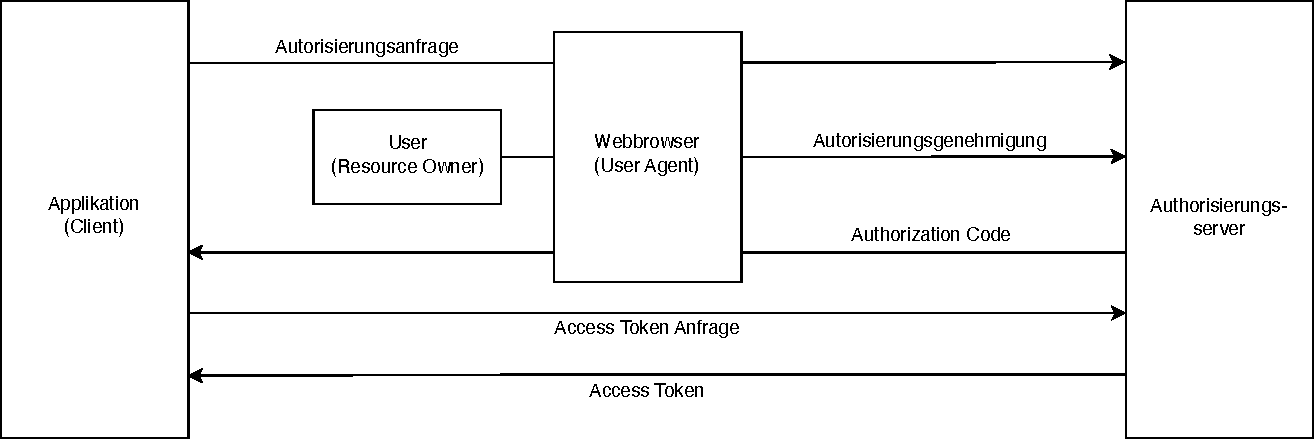
\includegraphics[width=\textwidth]{Authentication_Code_Grant.pdf}
\caption{Ablauf des Authentication Code Grant}
\label{fig:auth-code-grant}
\end{figure}

\section{OpenID Connect}
\label{auth:openid}

OpenID Connect ist eine Spezifikation, wie \textit{ID Tokens} mit personenbezogenen Daten ausgegeben werden \cite{OpenID.Core}. 
Dabei setzt OpenID Connect auf das OAuth2-Protokoll auf. 
OpenID Connect definiert ein weiteren \textit{response$\_$type=id$\_$token}. 
Dieser ermöglicht es, neben dem Access Token den sogenannten \textit{ID Token} in Form eines JSON Web Tokens \cite{rfc7519} vom Autorisierungsserver anzufordern. 
Um OpenID Connect nutzen zu können, muss im in \refabschnitt{auth:oauth2} beschriebenen Autorisierungsprozess der Parameter \textit{Scopes} um \textit{openid} erweitert werden. \\

Über den ID Token erlangt der Client Zugriff auf personenbezogene Daten des Benutzers. 
\textit{OpenID Connect} definiert eine Reihe von Standard-\textit{claims} \cite[Abschnitt~StandardClaims]{OpenID.Core}), die im \textit{Scope}-Parameter beim Aufruf der Autorisierungs-URL aufgelistet werden. 
Standard-\textit{claims} können um Custom-\textit{claims} erweitert werden, um die gewünschten Benutzerinformationen im ID Token angefordern.


\section{Einschränkung der Daten}
\label{auth:limit_data}

Die Spezifikation der REST-API sieht vor, dass die Sichtbarkeit der Daten an den definierten Endpunkte bereits im JSON-Objekt gemäß der Berechtigung des anfragenden Benutzers berücksichtigt ist. 
Daher muss der \textit{ID Token} Informationen enthalten, über die der IdM-Provider den Benutzer eindeutig identifizieren kann.
Die Informationen aus dem ID Token reichen ggf. jedoch nicht aus, um die Sichtbarkeit der Daten korrekt zu beschränken, da einem Benutzer im IdM mehrere Schule-Rolle-Kombinationen zugewiesen sein können (z.B. Tätigkeit als Lehrkraft an verschiedenen Schulen oder sowohl Lehrkraft als auch Elternteil eines Schülers an derselben Schule). 
Daher muss die Information, mit welcher Kombination von Schule und Rolle innerhalb dieser Schule der Aufruf eines REST-API-Endpunkts durchgeführt wird, an den IdM-Provider übermittelt werden. 
Dies geschieht durch die Erweiterung der \textit{Scopes}-Liste um den Scope für die Schule und die Rolle als Parameterübergabe beim Autorisierungsvorgang. 
\reflisting{listing:authorization_request} zeigt einen exemplarischen Aufruf des \textit{Authorization Endpoints} mit Übergabe der \textit{Scopes}.
Die zusätzlichen \textit{Scopes} für Schule und Rolle sind somit im Access Token hinterlegt und können bei der Generierung des zurückzuliefernden JSON-Objekts verwendet werden.

\begin{lstlisting}[caption={Beispielhafter Aufruf des Authorization Endpoints},label={listing:authorization_request},frame=tlrb]
https://<URL zum Authorization Endpoint>?response_type=code
&client_id=<Identifier von Client-App>
&redirect_uri=<Redirect-URL>
&scope=openid teacher school
&state=<Undurchschaubarer Wert fuer Sicherheitszwecke>
\end{lstlisting}

Ein Sonderfall stellen dabei Benutzerkonten mit der Rolle ''sync-system'' dar. 
Diese haben bei Aufruf eines REST-API-Endpunkts grundsätzlich keine Beschränkung auf eine einzelne Schule. 
Daher muss beim Autosierungsvorgang auch kein \textit{Scope} für die Schule an den Autorisierungsserver übergeben werden. \\

Sofern für ein Benutzerkonto im IdM mehrere Schule-Rolle-Kombinationen hinterlegt sein können, müssen Schule und Rolle bei Start des Authentifizierungsprozesses gegebenenfalls durch den Benutzer wählbar sein. 
Für einen Schule-Rolle-Wechsel ist eine Neuanmeldung bzw. Aktualisierung des Access Tokens bezüglich der \textit{Scopes} für Schule und Rolle notwendig.